\documentclass[aspectratio=169]{beamer}
\usetheme{metropolis}
\usepackage[british]{babel}
\usepackage{amsmath}
\usepackage{graphicx}
\usepackage{booktabs}
\usepackage{makecell}
\setbeamerfont{title}{size=\Large}

% Compile from deliveries/presentation, for example with latexmk -pdf presentation.tex.
\graphicspath{{../../deliverables/report/}}

\title{Regularized GLM--Neural Network Hybrids for Insurance Pricing}
\subtitle{CAS ETH in Machine Learning in Finance and Insurance\\Innovation Project}
\author{Leonhard Vogt}
\date{6 November 2026}

\begin{document}

\begin{frame}[plain,shrink=10]
    \titlepage
\end{frame}

\begin{frame}{Research question}
    Can jointly training a generalised linear model (GLM) and a regularized
    neural correction preserve predictive performance while favouring
    a more interpretable structure?

    \medskip
    \begin{itemize}
        \item Train both branches jointly, penalising the neural
        dense-layer weights while leaving the GLM unpenalised.
        \item Examine predictive fit, GLM coefficients and the neural
        contribution along the regularization path.
    \end{itemize}
\end{frame}

\begin{frame}{Regularized mixed GLM-FNN data flow}
    \centering
    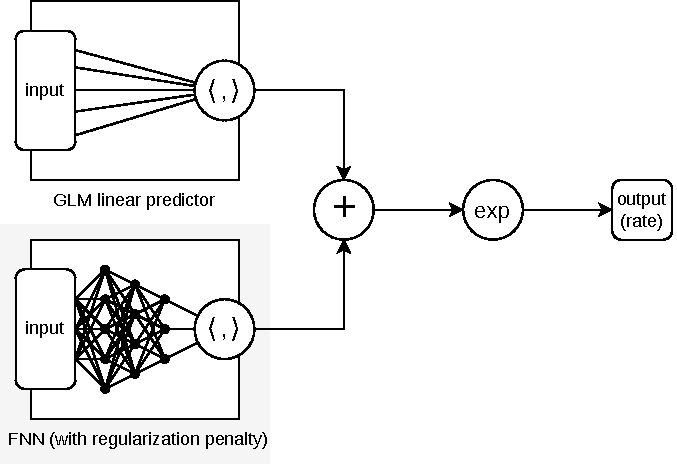
\includegraphics[width=\textwidth,height=0.75\textheight,keepaspectratio]{mixed.drawio.pdf}
\end{frame}

\begin{frame}{GLM data flow}
    \centering
    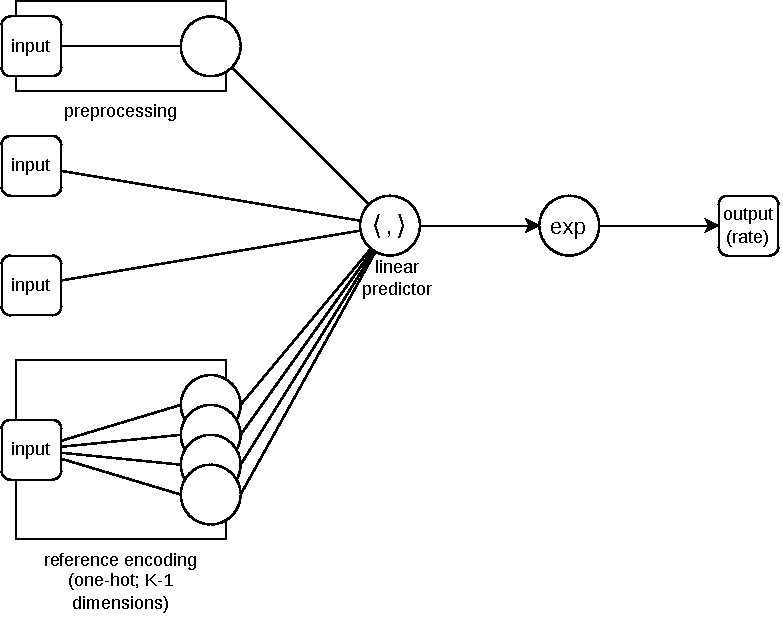
\includegraphics[width=\textwidth,height=0.75\textheight,keepaspectratio]{glm.drawio.pdf}
\end{frame}

\begin{frame}{Input preprocessing for the linear and neural branches.}
    \centering
    \small
\begin{tabular}{@{}p{0.20\linewidth}p{0.34\linewidth}p{0.36\linewidth}@{}}
\toprule
Feature & GLM branch & Neural branch\\
\midrule
Driver age & 7 groups, dummy encoded & Capped at 90; standardised\\
Vehicle brand & Dummy encoding & Two-dimensional embedding\\
Fuel type & Dummy encoding & Dummy encoding\\
Population \mbox{density} & Natural logarithm & Logarithm rounded to two decimals; standardised\\
Area & Ordinal codes one to six & Ordinal codes; standardised\\
Vehicle age & Omitted & Capped at 20; standardised\\
Bonus--malus & Omitted & Capped at 150; standardised\\
Vehicle power & Omitted & Capped at 15; standardised\\
Region & Omitted & Two-dimensional embedding\\
\bottomrule
\end{tabular}
\end{frame}

\begin{frame}{Implementation challenges}
    \small
    \begin{itemize}
        \item Represent the GLM as a trainable Keras layer so that stochastic gradient descent can
        update both branches jointly.
        \item Transfer the fitted GLM coefficients at initialisation.
        \item Control optimisation drift from the maximum likelihood
        estimates through batch-size and epoch choices.

        \item Omit the neural output bias to avoid duplicating the GLM
        intercept.
    \end{itemize}
\end{frame}



\begin{frame}{GLM in Keras}
    \centering
    \resizebox{\textwidth}{!}{%
\begin{tabular}{l r r c r r r r}
\toprule
Model Name & \makecell{Batch\\Size} & \makecell{Epochs} & Split & \makecell{Train\\Dev.} & \makecell{Train\\Cal.} & \makecell{Test\\Dev.} & \makecell{Test\\Cal.} \\
\midrule
GLM (statsmodels) & - & - & - & 46.9537 & 1.0000 & 47.1786 & 0.9978 \\
Keras Control & - & - & - & 46.9537 & 1.0000 & 47.1786 & 0.9978 \\
Keras Trained & 5\,000 & 200 & 90/10 & 47.0045 & 1.0338 & 47.2504 & 1.0313 \\
Keras Stability Test & 5\,000 & 20 & 90/10 & 46.9668 & 1.0388 & 47.1970 & 1.0367 \\
Keras Trained & 5\,000 & 200 & - & 46.9612 & 1.0095 & 47.2000 & 1.0072 \\
Keras Trained & 50\,000 & 2\,000 & - & 46.9545 & 1.0026 & 47.1742 & 1.0003 \\
Keras Trained & 50\,000 & 2\,000 & 90/10 & 46.9887 & 0.9943 & 47.2329 & 0.9918 \\
\bottomrule
\end{tabular}
    }
\end{frame}



\begin{frame}{FNN data flow}
    \centering
    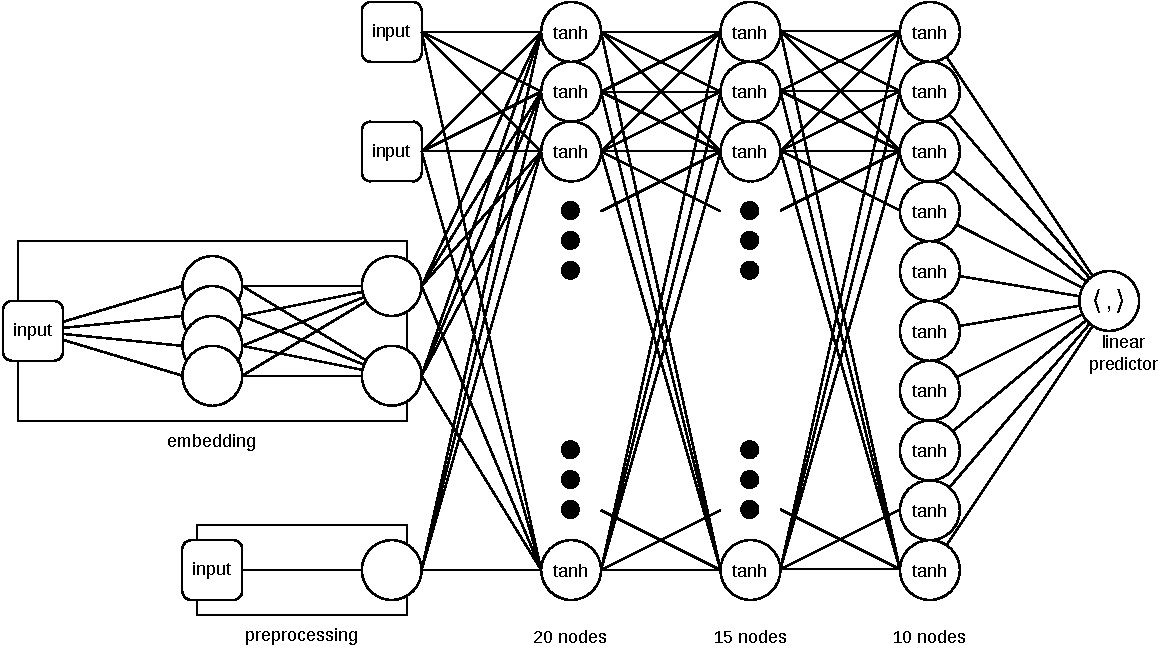
\includegraphics[width=\textwidth,height=0.75\textheight,keepaspectratio]{fnn.drawio.pdf}
\end{frame}

\begin{frame}{CANN data flow}
    \centering
    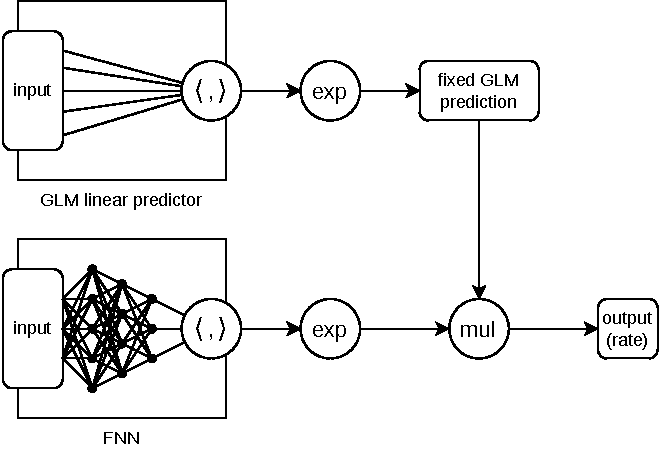
\includegraphics[width=\textwidth,height=0.75\textheight,keepaspectratio]{cann.drawio.pdf}
\end{frame}

\begin{frame}{Regularized mixed GLM-FNN data flow}
    \centering
    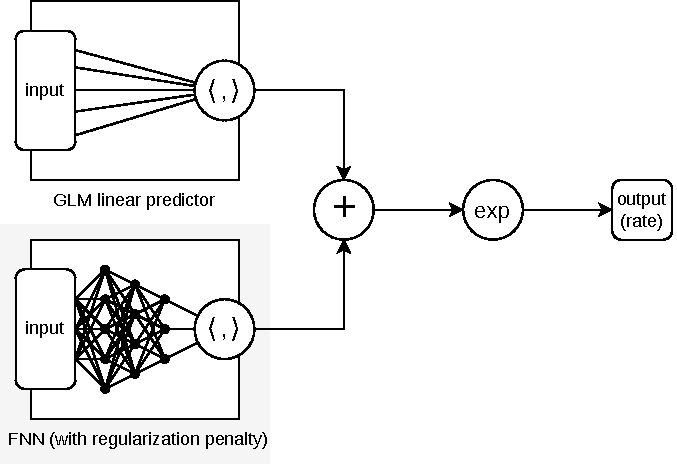
\includegraphics[width=\textwidth,height=0.75\textheight,keepaspectratio]{mixed.drawio.pdf}
\end{frame}

\begin{frame}{Selected saved notebook results}
    \centering
    \small
\begin{tabular}{lrrr}
\hline
Model & Learning $D_{100}$ & Test $D_{100}$ & Test O/E\\
\hline
GLM & 46.954 & 47.179 & 0.9978\\
Keras GLM control & 46.954 & 47.179 & 0.9978\\
Frozen CANN & 44.970 & 44.955 & 1.0103\\
FNN & 44.830 & 44.894 & 1.0163\\
FNN, mean initialisation & 44.814 & 44.902 & 1.0229\\
Joint hybrid, $\lambda=0$ & 44.986 & 44.989 & 0.9964\\
Joint hybrid, $\lambda=10^{-5}$ & 45.011 & 44.952 & 1.0028\\
Joint hybrid, $\lambda=1$ & 46.955 & 47.182 & 0.9966\\
\hline
\end{tabular}

    \footnotesize
    Batch sizes differ between benchmarks and hybrids.
\end{frame}



\begin{frame}{Regularization path of the jointly trained hybrid}
    \centering
    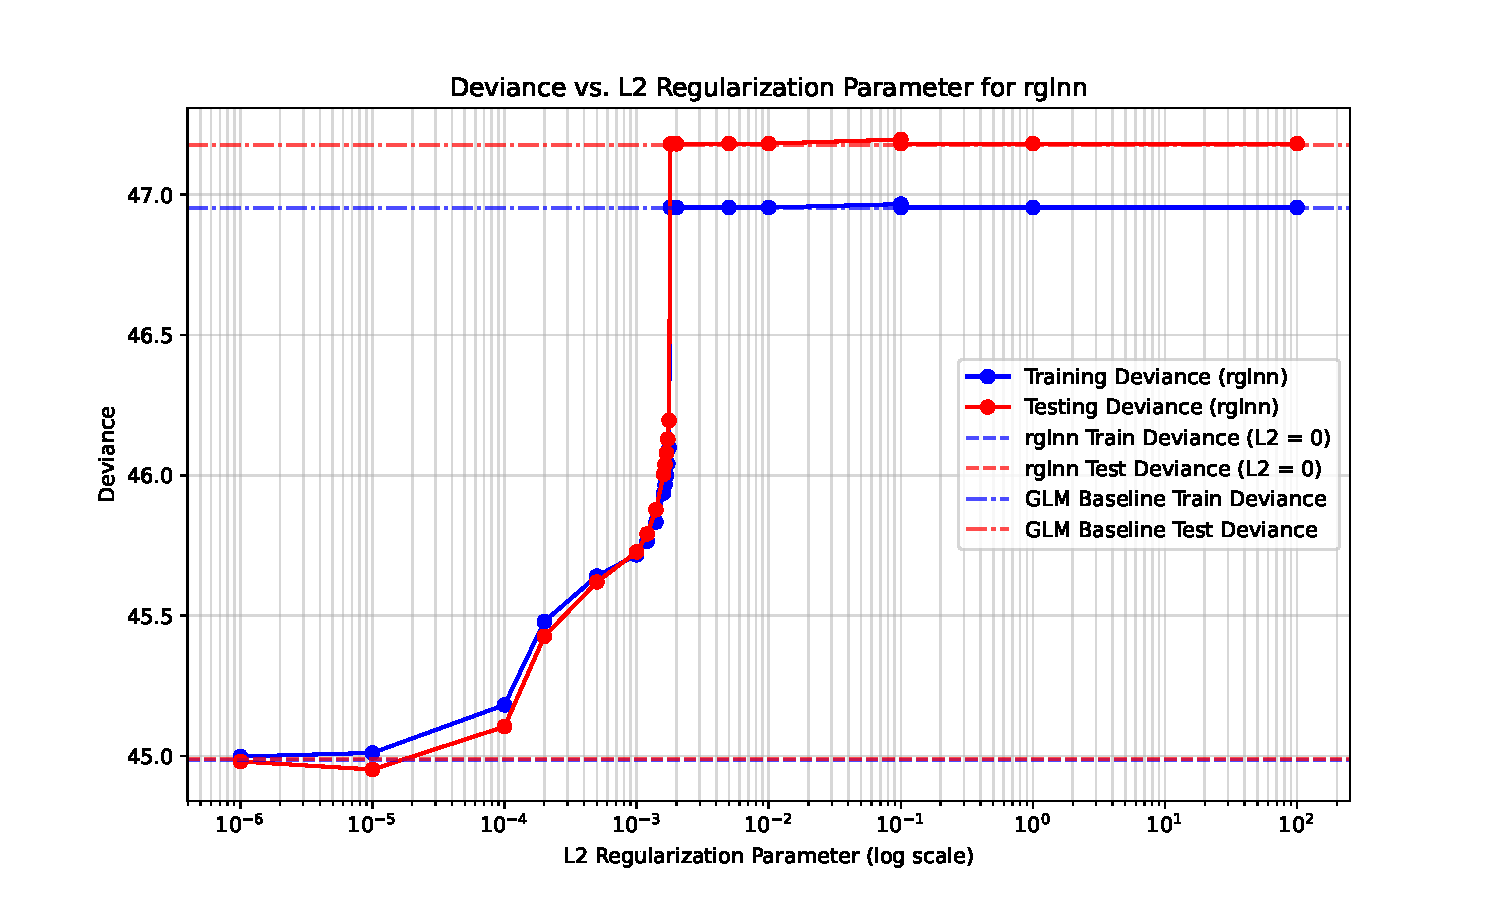
\includegraphics[width=\textwidth,height=0.75\textheight,keepaspectratio]{results/deviance_vs_reg.pdf}
\end{frame}

\begin{frame}{GLM parameters for selected features for different regularization strengths}
    \centering
    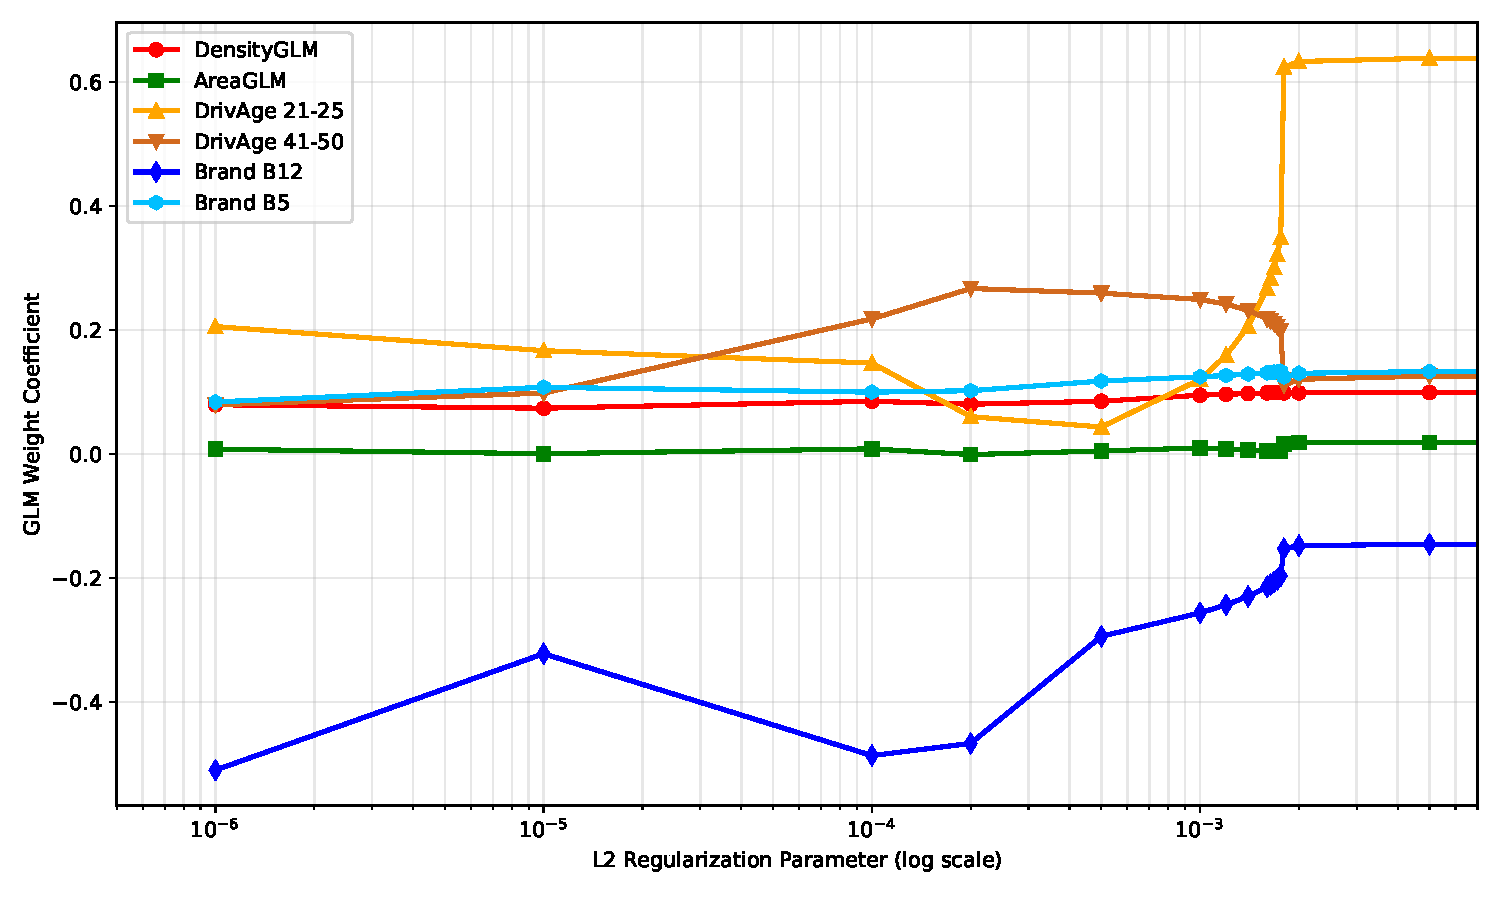
\includegraphics[width=\textwidth,height=0.75\textheight,keepaspectratio]{results/glmbeta_vs_reg.pdf}
\end{frame}

\begin{frame}{FNN correction in regularized model}
    \centering
    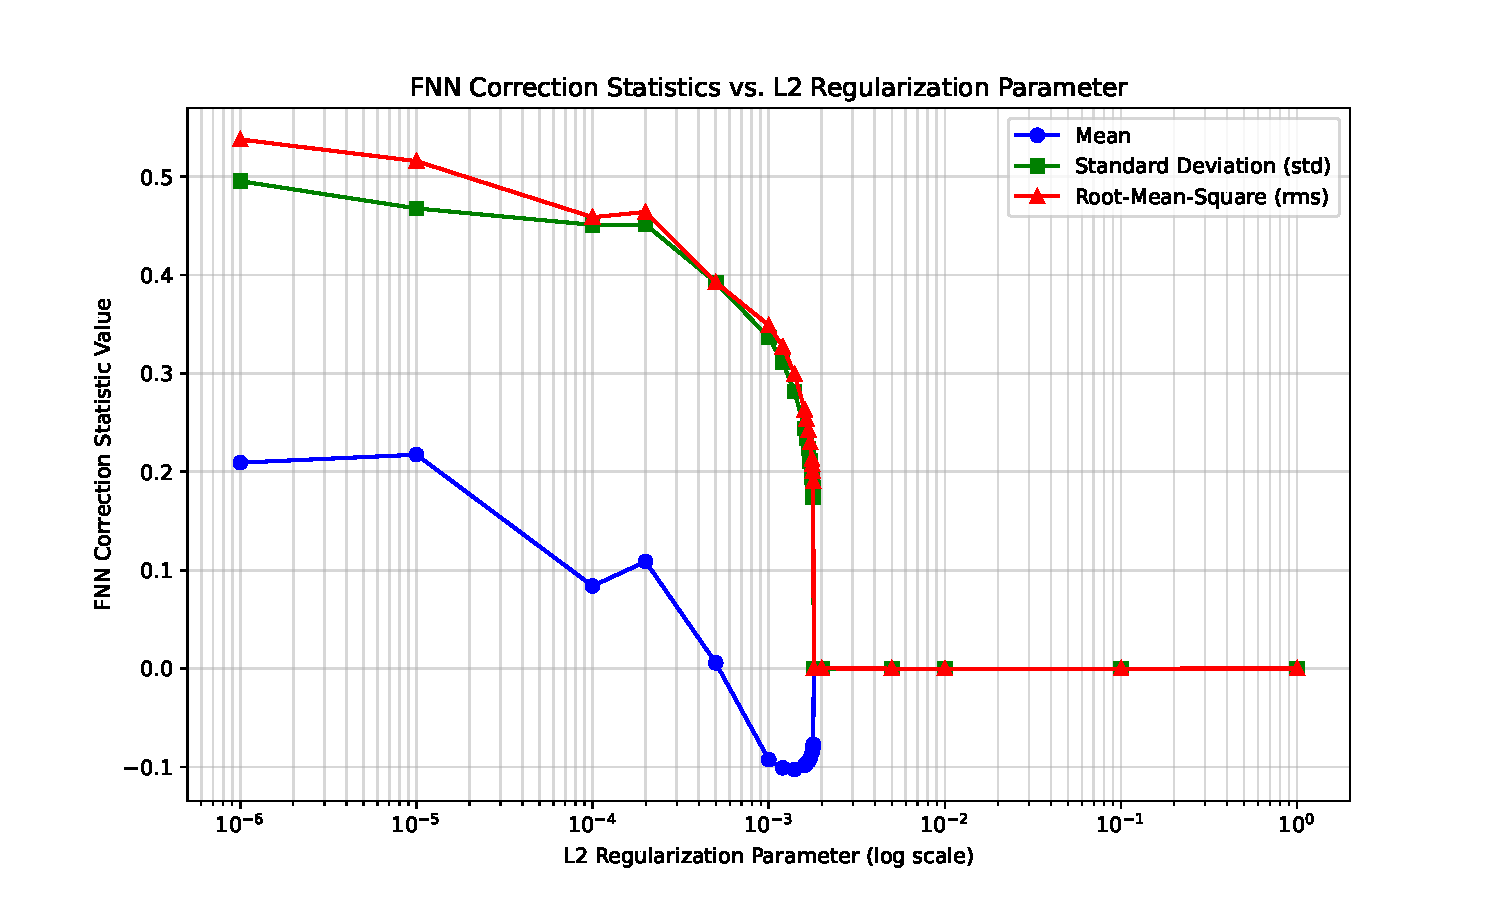
\includegraphics[width=\textwidth,height=0.75\textheight,keepaspectratio,trim=0 0 0 24pt,clip]{results/fnn_correction_stats.pdf}
\end{frame}

\begin{frame}{FNN correction in regularized model - Histograms}
    \centering
    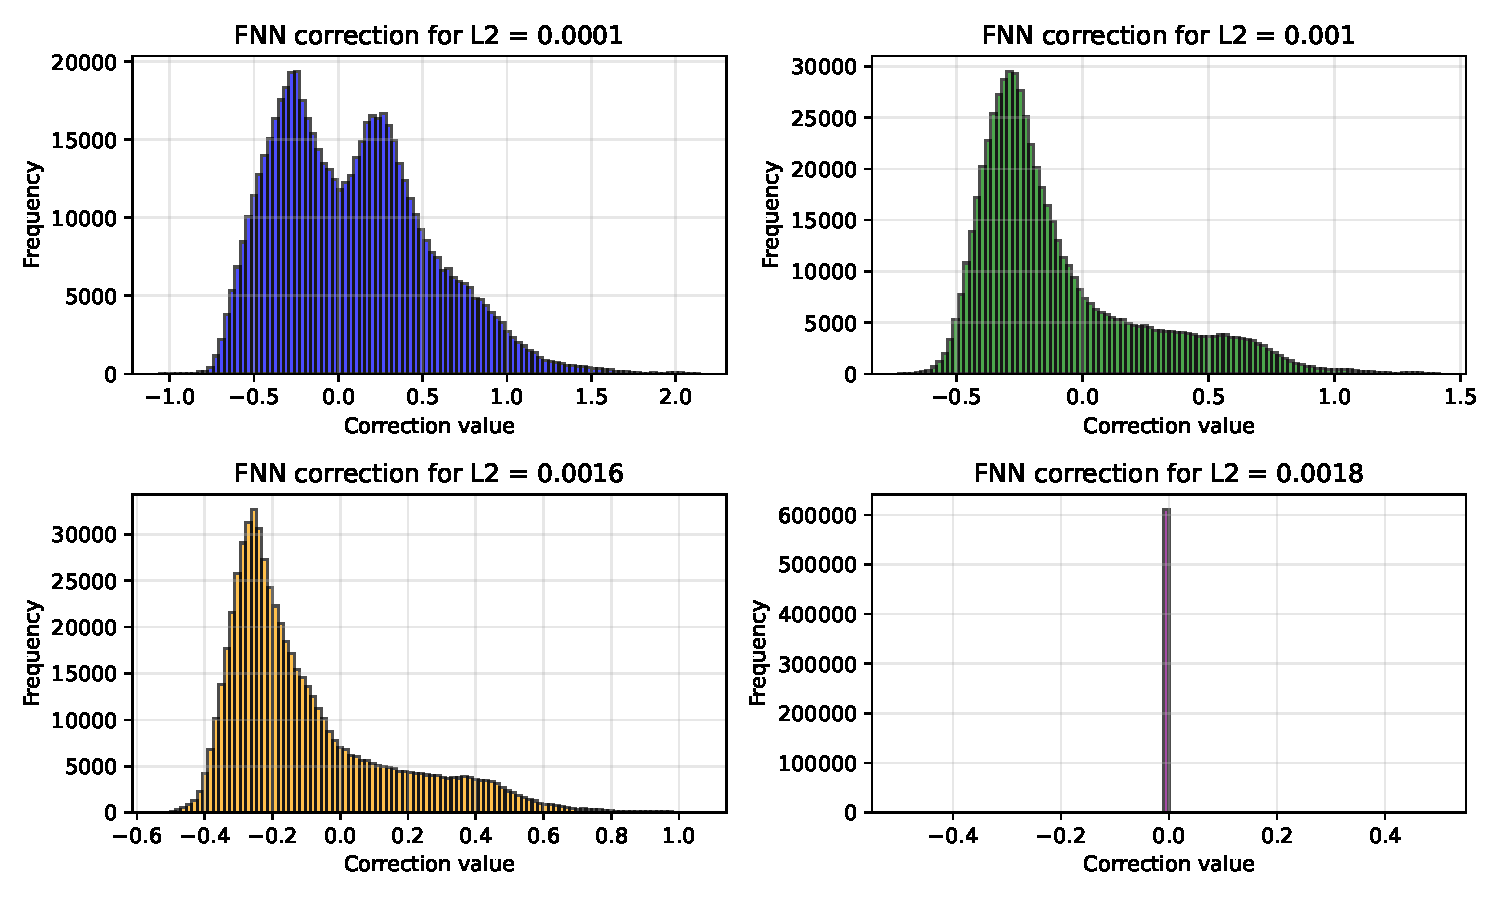
\includegraphics[width=\textwidth,height=0.75\textheight,keepaspectratio]{results/fnn_correction_histograms.pdf}
\end{frame}

\begin{frame}{Real-world applicability}
    \small
    \begin{itemize}
        \item A regularization path shows how much predictive accuracy can be gained by adding complexity to a simpler GLM.
        \item Joint training allows the linear tariff component to adapt.
        \item The neural network makes substantial contributions to the GLM predictions before the sharp transition.
        \item Practical use needs subgroup calibration, stability checks, documented pricing decisions and costs beyond claim frequency.
    \end{itemize}
\end{frame}

\begin{frame}{Lessons learned}
    \small
    \begin{itemize}
        \item Regularization controls the neural contribution, but the
        transition towards GLM-like predictions is abrupt.
        \item The hybrid model does not imply interpretability like a GLM, as
        both branches substantially contribute to predictions up to the transition point.
        \item Stochastic optimisation
        can move a fitted GLM away from its maximum likelihood estimates. Sufficient batch size alleviates this issue.
        \item Hybrids retain GLM feature-design choices and neural-network
        tuning, with regularization strength as an additional choice, thus combining challenges of both approaches.
        \item Predictive fit and calibration need separate assessment, assess both when selecting models.
    \end{itemize}
\end{frame}

\appendix
\begin{frame}[plain,noframenumbering]
    \centering
    \LARGE Appendix
\end{frame}

\begin{frame}{GLM in Keras}
    \centering
    \resizebox{0.72\textwidth}{!}{\begin{tabular}{l r r c r r r r}
\toprule
Model Name & \makecell{Batch\\Size} & \makecell{Epochs} & Split & \makecell{Train\\Dev.} & \makecell{Train\\Cal.} & \makecell{Test\\Dev.} & \makecell{Test\\Cal.} \\
\midrule
GLM (statsmodels) & - & - & - & 46.9537 & 1.0000 & 47.1786 & 0.9978 \\
Keras Control & - & - & - & 46.9537 & 1.0000 & 47.1786 & 0.9978 \\
Keras Trained & 5\,000 & 200 & - & 46.9612 & 1.0095 & 47.2000 & 1.0072 \\
Keras Stability Test & 5\,000 & 20 & - & 46.9560 & 1.0110 & 47.1885 & 1.0088 \\
Keras Trained & 5\,000 & 200 & 90/10 & 47.0045 & 1.0338 & 47.2504 & 1.0313 \\
Keras Stability Test & 5\,000 & 20 & 90/10 & 46.9668 & 1.0388 & 47.1970 & 1.0367 \\
Keras Trained & 50\,000 & 2\,000 & - & 46.9545 & 1.0026 & 47.1742 & 1.0003 \\
Keras Stability Test & 50\,000 & 200 & - & 46.9544 & 1.0026 & 47.1738 & 1.0004 \\
Keras Trained & 50\,000 & 2\,000 & 90/10 & 46.9887 & 0.9943 & 47.2329 & 0.9918 \\
Keras Stability Test & 50\,000 & 200 & 90/10 & 46.9546 & 0.9987 & 47.1820 & 0.9966 \\
Keras Trained & 200\,000 & 4\,000 & - & 46.9846 & 0.9965 & 47.1970 & 0.9939 \\
Keras Stability Test & 200\,000 & 400 & - & 46.9647 & 0.9988 & 47.1670 & 0.9965 \\
Keras Trained & 200\,000 & 4\,000 & 90/10 & 47.2781 & 0.9657 & 47.5141 & 0.9631 \\
Keras Stability Test & 200\,000 & 400 & 90/10 & 46.9547 & 1.0028 & 47.1832 & 1.0007 \\
\bottomrule
\end{tabular}
}
\end{frame}

\begin{frame}{Joint-hybrid sweep with batch size 50,000 and 200 epochs.}
    \centering
    \small
\begin{tabular}{rrrr}
\hline
$\lambda$ & Learning $D_{100}$ & Test $D_{100}$ & Test O/E\\
\hline
$0$ & 44.986 & 44.989 & 0.9964\\
$10^{-5}$ & 45.011 & 44.952 & 1.0028\\
$10^{-4}$ & 45.182 & 45.104 & 1.0118\\
$5\times10^{-4}$ & 45.641 & 45.620 & 0.9972\\
$10^{-3}$ & 45.717 & 45.727 & 0.9974\\
$2\times10^{-3}$ & 46.954 & 47.182 & 0.9961\\
$5\times10^{-3}$ & 46.955 & 47.182 & 0.9966\\
$10^{-2}$ & 46.955 & 47.182 & 0.9966\\
$10^{-1}$ & 46.955 & 47.182 & 0.9966\\
$1$ & 46.955 & 47.182 & 0.9966\\
\hline
\end{tabular}
\end{frame}

\end{document}
